The main goal of the Single-Phase Prototype test beam program is to perform measurements 
needed to control and understand systematic uncertainties in DUNE oscillation measurements.
The program also includes measurements to support other important DUNE physics measurements as described below.
%detector is intended to provide input necessary to reduce systematic uncertainties for oscillation measurements 
%

%Current assumptions on detector related systematic uncertainties in DUNE to achieve
%projected sensitivities~\cite{DuneCDR} are shown in
%%Assumptions on current level of uncertainties are shown in 
%Table \ref{table:deterr}. These are compared with teh levels achieved in MINOS and T2K
%appearance measurements.
%\begin{table}[h]
%\centering
%\caption{Current estimated detector related  sources of uncertainty for oscillation 
%measurements.}
%\label{table:deterr}
%\begin{tabular}{|l|c|c|c|l|}
%\hline
%\textbf{Source of uncertainty } & \textbf{MINOS} & \textbf{T2K} & \textbf{DUNE} & \textbf{Comments}  \\ \hline
%$\nu_e$ energy scale  & 2.7\% & 2.5\% & 2\% & comment \\ \hline
%\end{tabular}
%\end{table}
%% THIS IS FROM TABLE 3.8 of CDR


As an example of the importance of controlling detector related uncertainties,
Fig.~\ref{fig:spectraleffect} shows the effect of a lepton energy scale 
uncertainty of 10\% on the measured 
appearance signal (for $\delta_{CP}=0$, etc.). 
and backgrounds in DUNE. The dashed curve (ADD CURVE) shows the expected signal shape
 for $\delta_{CP}=?$. Energy scale uncertainties can mimic a non-zero
$\delta_{CP}$ phase. 
\begin{figure}[h!]
\centering
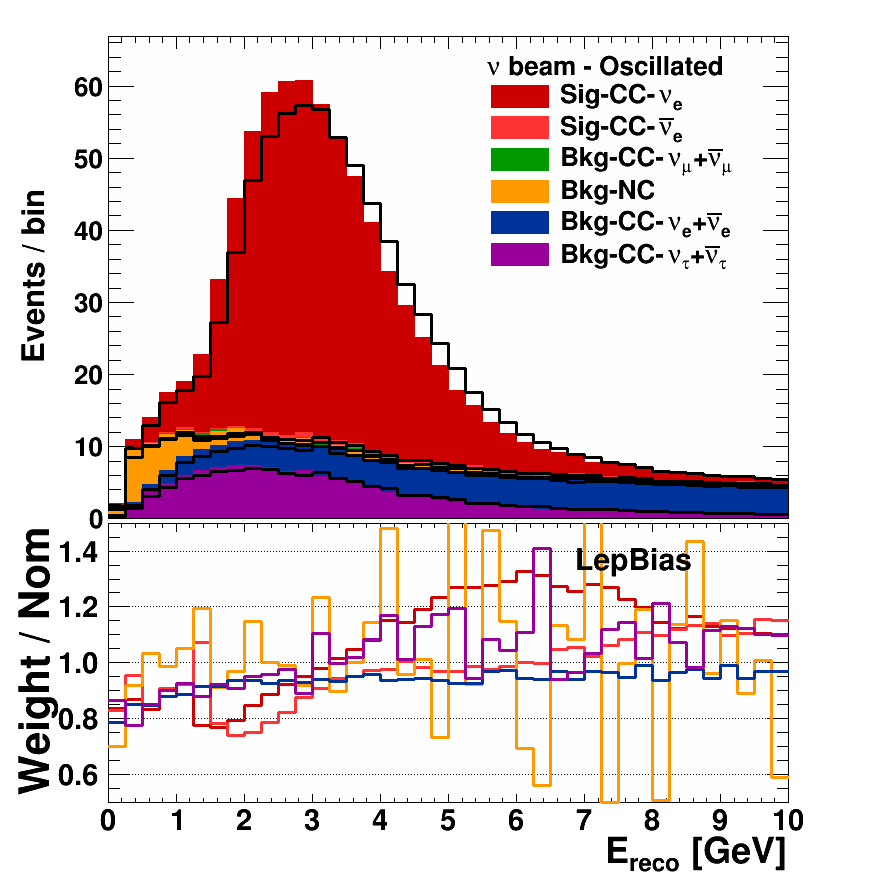
\includegraphics[width=0.7\textwidth,height=7.7cm]{figures/lepbias10}
\label{fig:spectraleffect}
  \caption{DUNE $\nu_e$ appearance signal and background spectra assuming 
$\delta_{CP}=0$. 
Solid curves shows the effect of 10\% lepton energy scale shift on the 
measured appearance signal 
and backgrounds. The dashed-curve (NEEDS TO BE ADDED) shows the 
expected signal shape for 
$\delta_{CP}=?$.
{\color{red} 
Need to add details of plot assumptions
}
}
\end{figure}
Effects on sensitivity to mass hierarchy and $\delta_{CP}$ as a function of 
$\delta_{CP}$ are shown in Fig.~\ref{fig:global_escale_sens} from Ref.~\cite{DUNECDR}. 
%shows the effect of various levels of neutrino energy on sensitivities. 
The nominal sensitivity assumes a 230-kt-MW-year 
exposure with equal neutrino and antineutrino mode running. 
This does not account for correlated uncertainties in neutrino and 
antineutrino running or effects on backgrounds and is therefore likely
a best-case scenario. 
\begin{figure}[h!]
\centering
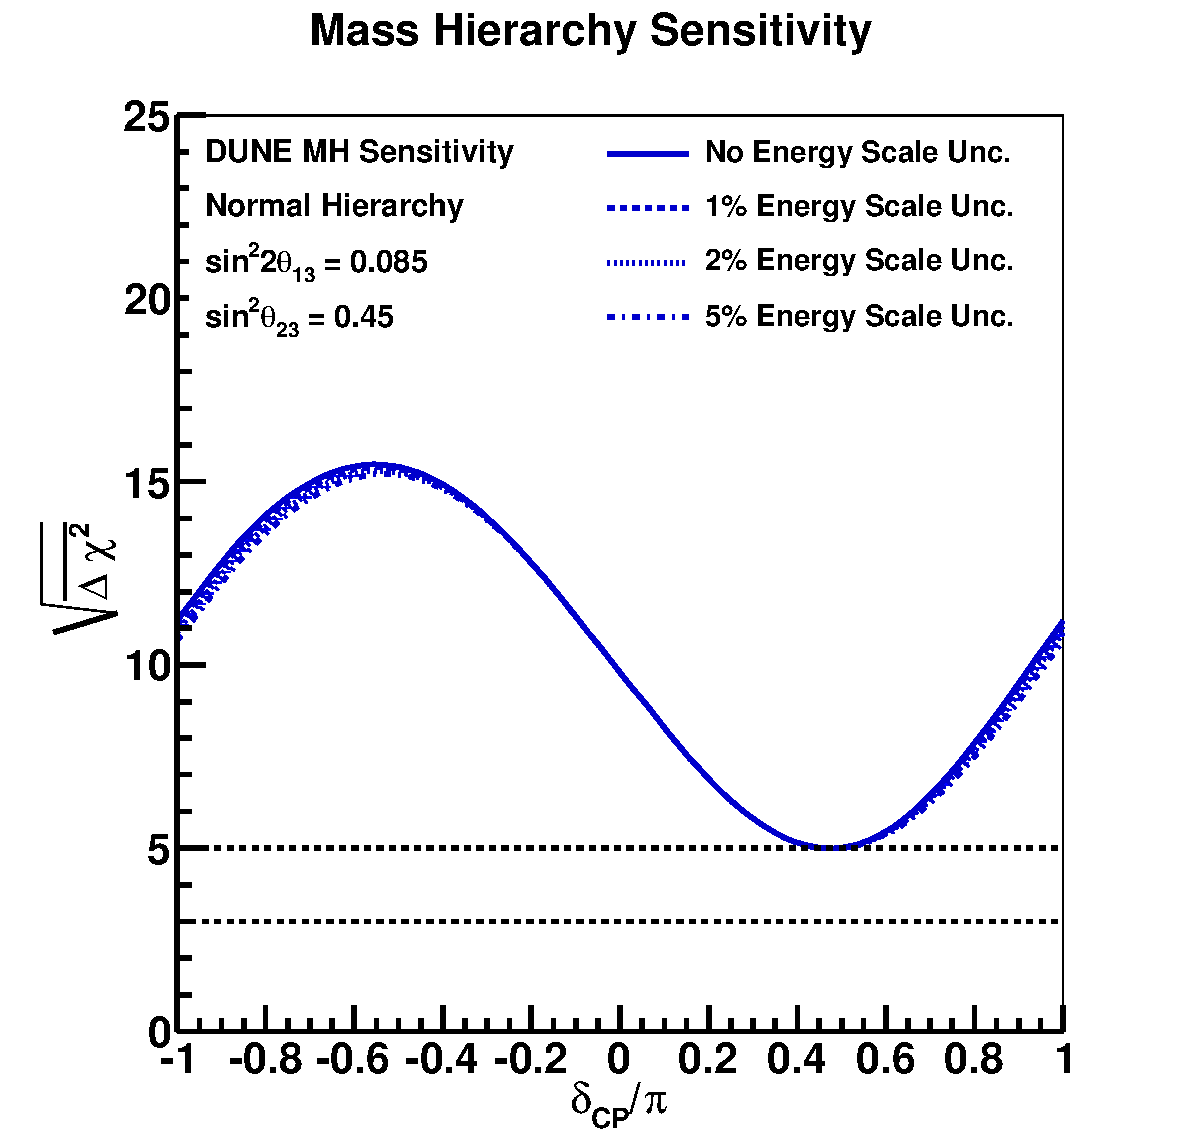
\includegraphics[width=0.49\textwidth,height=6.7cm]{figures/mh_230ktmwyear_varyesyst}
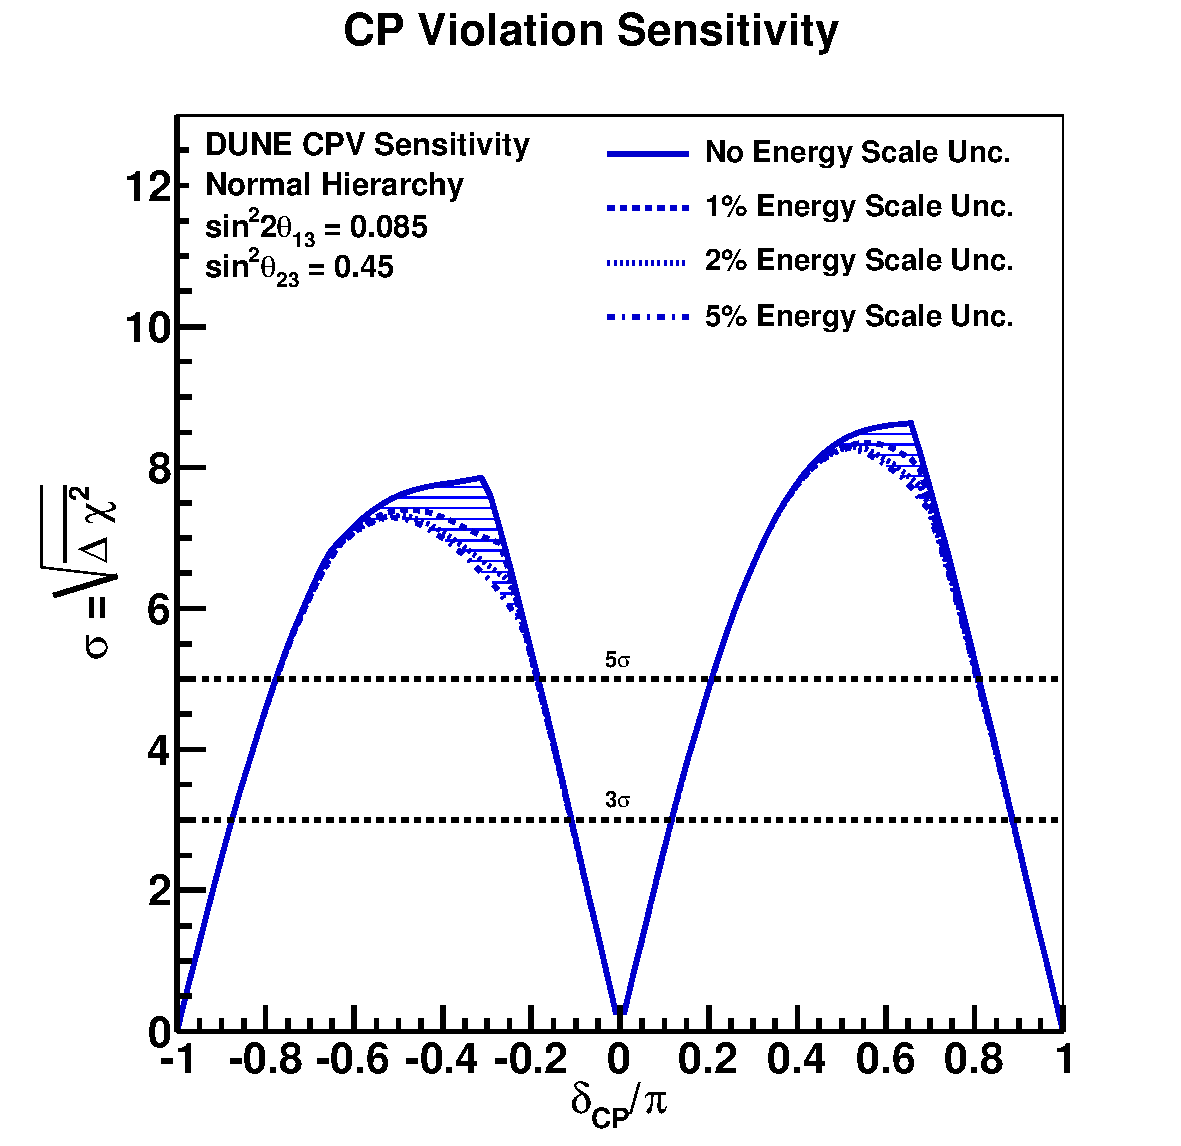
\includegraphics[width=0.49\textwidth,height=6.7cm]{figures/cpv_890ktmwyear_varyesyst}
%\includegraphics[width=0.49\textwidth,height=6.7cm]{figures/mh_escale_sens}
%\includegraphics[width=0.49\textwidth,height=6.7cm]{figures/deltacp_escale_sens}
\label{fig:global_escale_sens}
  \caption{DUNE projected sensitivity dependence of mass hierarchy (left) and $\delta_{CP}$ 
(right) to neutrino energy scale uncertainties. 
If energy scale uncertainties can be controlled at the appropriate levels, DUNE can achieve 
at least 5$\sigma$ sensitivity on mass hierarchy determination for 100\% of $\delta_{CP}$ values and
for 3$\sigma$ sensitivity to  $\delta_{CP}$ for 75\% coverage of phase space.
{\color{red} 
Need to check details of assumptions
}
}
\end{figure}

Work to evaluate effect of all systematic uncertainties in DUNE sensitivities is still in progress. Current levels of sensitivity in ~\cite{DuneCDR} assumes
$\nu_e$ energy scale is known at the level of 2\%. 
More here...
%will require a dedicated test beam


%$\nu_e$ energy scale  & 2.7\% & 2.5\% & 2\% & comment \\ \hline
%\end{tabular}


\subsection{Summary of Detector and Beam Requirements }
\label{detbeam_main}

LAr TPC technology was first proposed for use in neutrino experiments by C. Rubbia in 1977
\cite{Rubbia} but extensive use in neutrino experiments is only now being realized. 
%CERN-EP-INT-77-8
%Title 	The liquid-argon time projection chamber : a new concept for neutrino detectors
%operating in the CNGS beamline  (with mean beam energy $\sim$17 GeV)~\cite{ICARUSmain}. 
The ICARUS T600 detector~\cite{ICARUSrefs} pioneered the first large-scale detector operating in the CNGS 
neutrino beam at mean energy $\sim$17 GeV. ArgoNEUT~\cite{argoneut} recently studied 
neutrino interactions in the NuMI beam down to sub-GeV energies with a small-scale (170~$l$ fiducial volume) detector. 
While these samples are proving useful, they do now allow full isolation of
the low energy neutrino interaction processes
and final states from reconstruction and detector effects. 
The use of this technology in future precision neutrino experiments will require dedicated 
information on particle response
in the few-GeV to sub-GeV range provided charged-particle test beams. 

%%%
%\subsubsection{Particles energy and direction}
%\label{detbeam_particles}
The DUNE experiment will run beam in both neutrino and anti-neutrino 
configurations. These beams will be composed  mainly of muon neutrinos (anti-neutrinos) as well as electron neutrinos (anti-neutrinos). In Fig. \ref{fig:particle_momenta} the distributions of momenta and angles of particles created in neutrino interactions from simulated beam fluxes are shown. 
\begin{figure}[h!]
  \centering
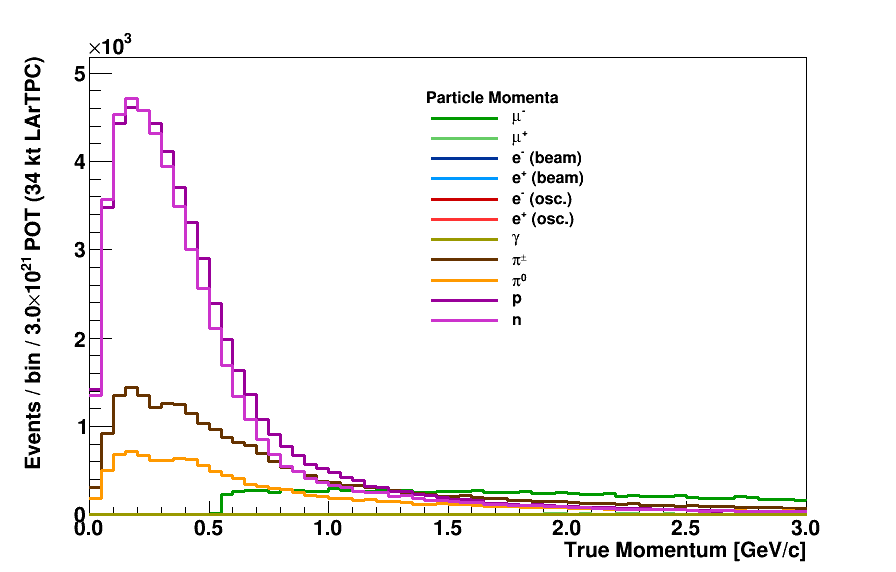
\includegraphics[width=0.49\textwidth,height=5.0cm]{figures/True_Momenta_per_Particle}
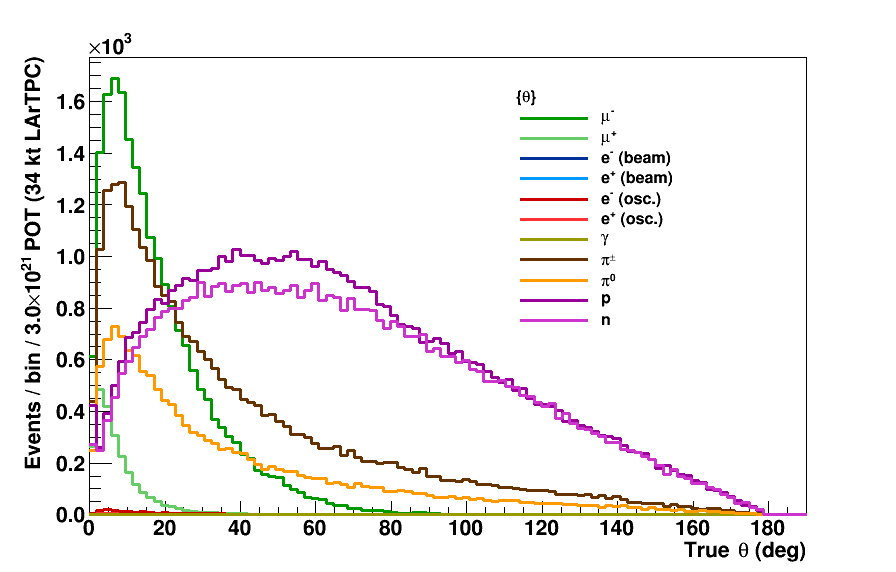
\includegraphics[width=0.49\textwidth,height=5.0cm]{figures/True_theta_per_Particle}
\label{fig:particle_momenta}
  \caption{Particle momenta (left) and angular (right) distributions for particles produced in neutrino interactions 
from $\nu_e$, $\nu_\mu$, $\bar \nu_e$ and $\bar \nu_\mu$ at the far detector location.
{\color{red}
Want y-log scale version - combine e+e-, fix mu, improve information content (y-axis, change colors, etc )
}
}
\end{figure}


%\begin{figure}[h!]
%  \centering
%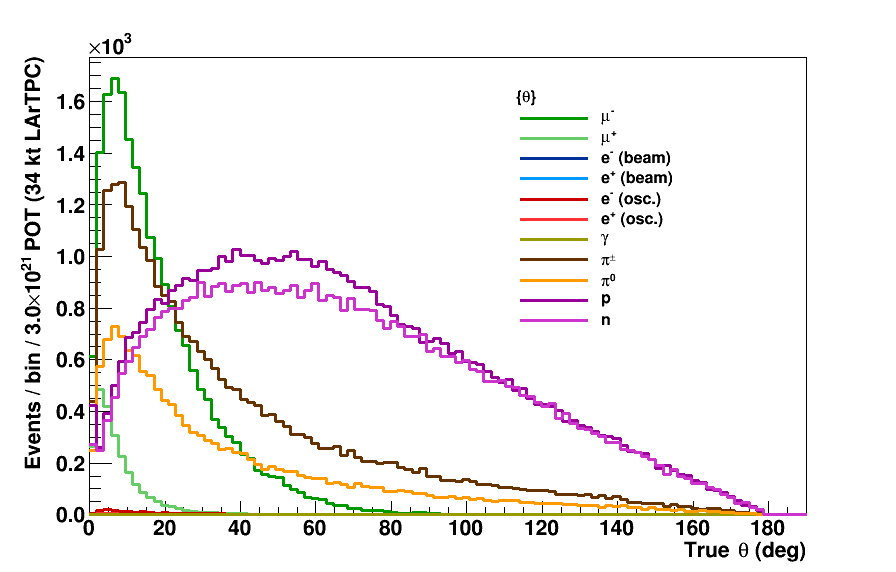
\includegraphics[scale=0.4]{figures/True_theta_per_Particle}
%\label{fig:particle_theta}
%  \caption{Particle angle wrt to the beam axis distributions for particles coming from all fluxes ($\nu_e$, $\nu_\mu$, $\bar \nu_e$ and $\bar \nu_\mu$) at both near and far detector locations.  }
%\end{figure}

%\newpage

The detector is designed to mimic the current DUNE Far detector design but must be sufficiently large in both
longitudinal and transverse dimensions to contain showering particles up to the energy range of interest ($\sim$7~GeV).
Fig.~\ref{fig:containment} shows the simulated longitudinal and transverse 
energy containment for proton showers up to 10~GeV/c momentum.
For 10 GeV showers, more than 95\% of the energy is contained in a detector of longitudinal size of 550~cm and 
radius of 200~cm. Shower from pions, kaons, and electrons have also been studied and better containment
is achieved in those cases. 
\begin{figure}[htp]
  \centering
  \label{fig:containment}  
  \begin{tabular}{ccc}
%    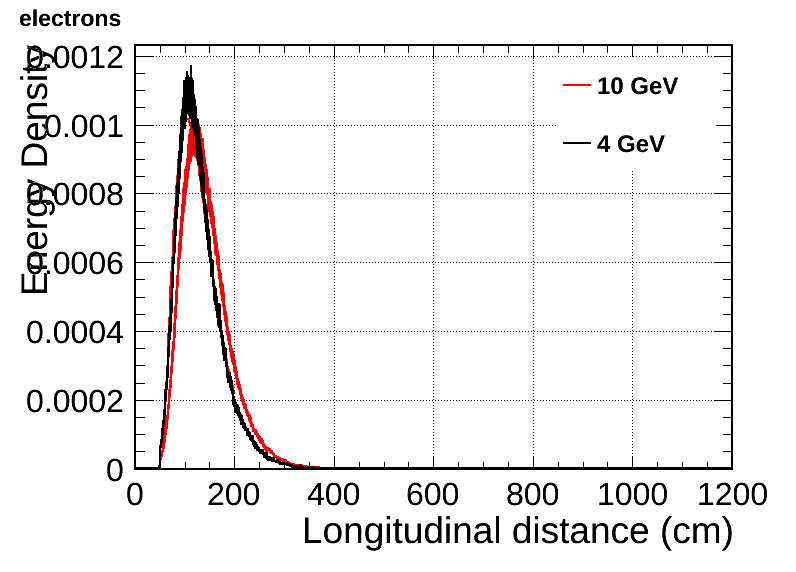
\includegraphics[scale=0.15]{figures/electrons_density_overlay}&
%    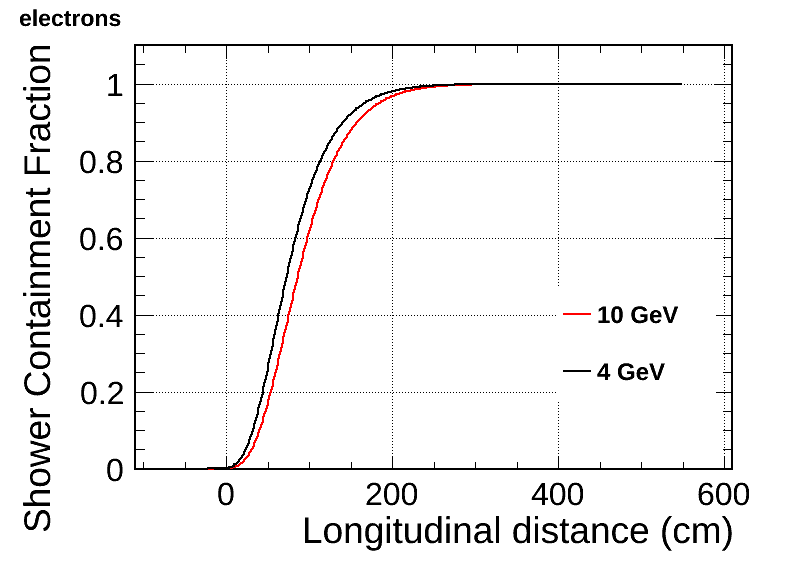
\includegraphics[scale=0.15]{figures/electrons_lcont_overlay}&
%    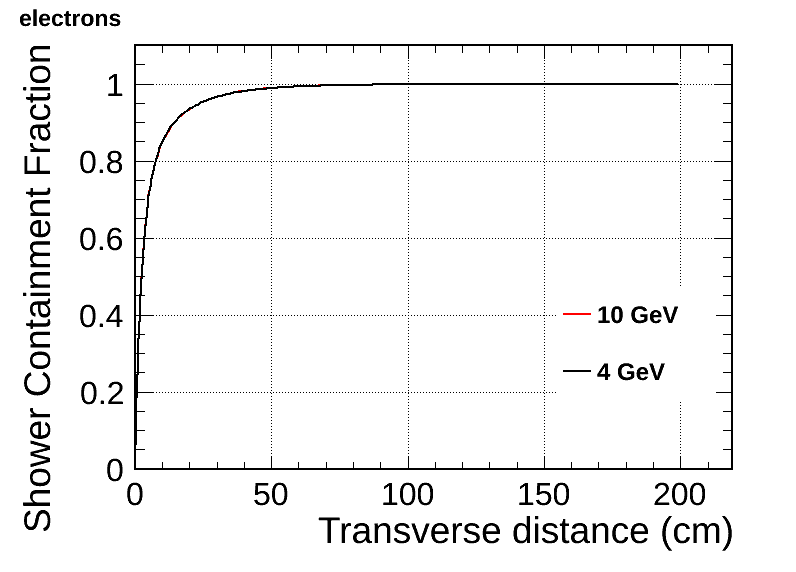
\includegraphics[scale=0.15]{figures/electrons_wcont_overlay}\\
%  
%    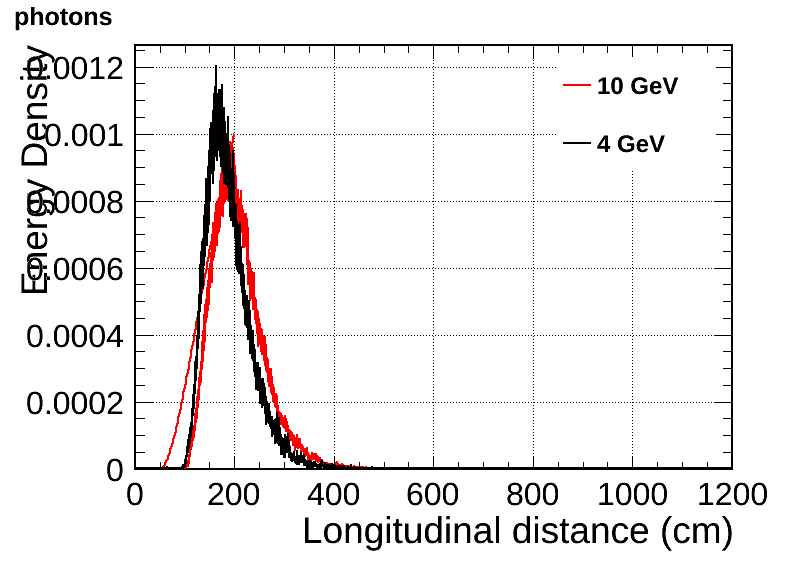
\includegraphics[scale=0.15]{figures/photons_density_overlay}&
%    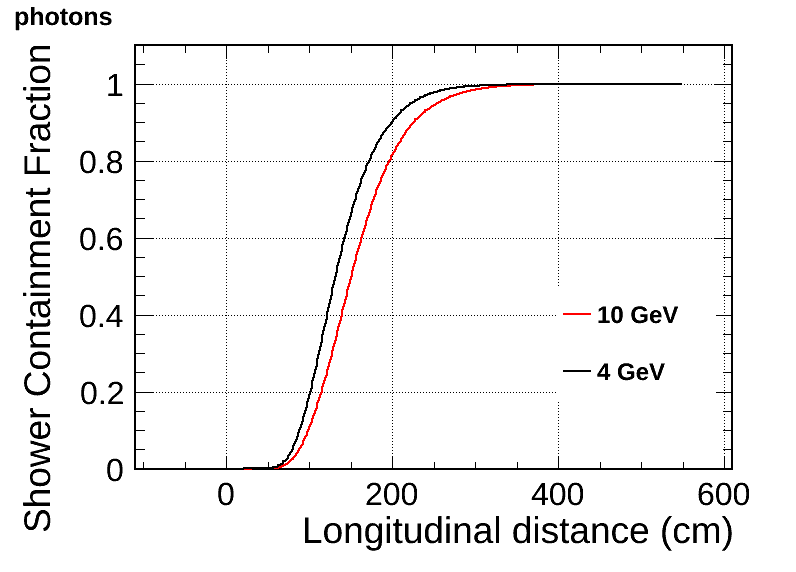
\includegraphics[scale=0.15]{figures/photons_lcont_overlay}&
%    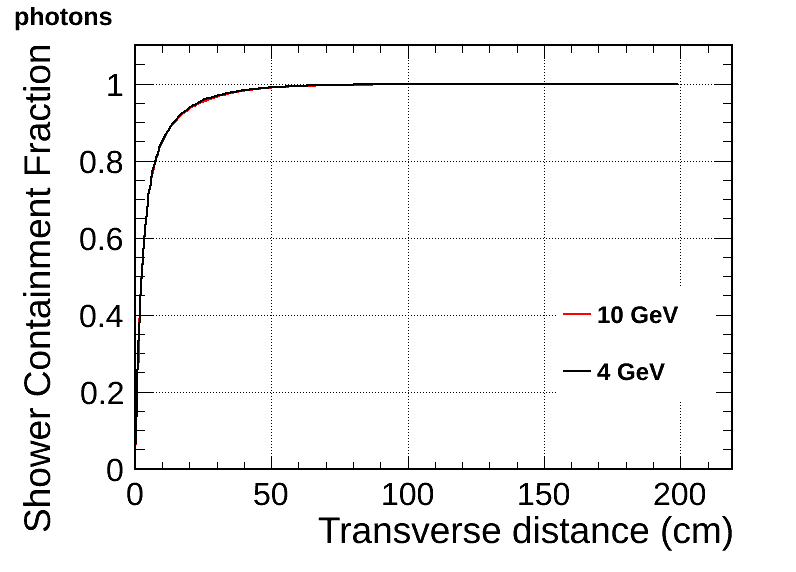
\includegraphics[scale=0.15]{figures/photons_wcont_overlay}\\
%%
%   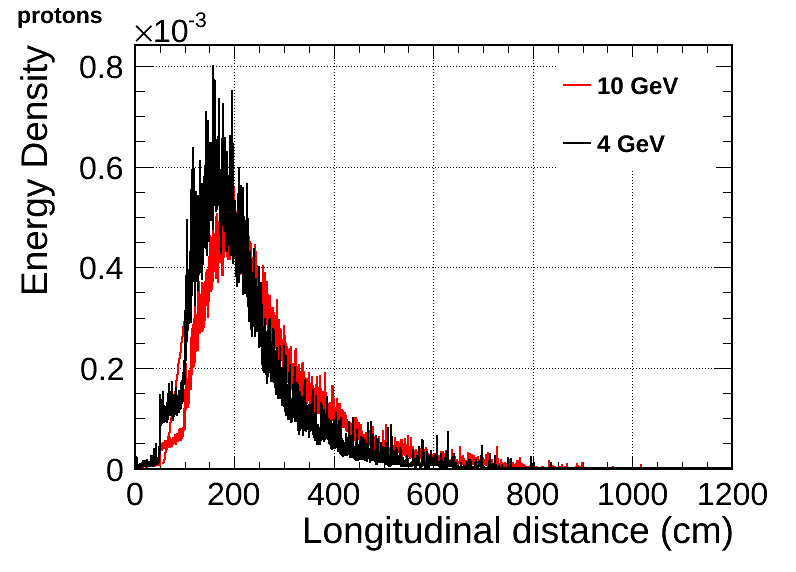
\includegraphics[width=0.31\textwidth,height=3.9cm]{figures/protons_density_overlay}&
   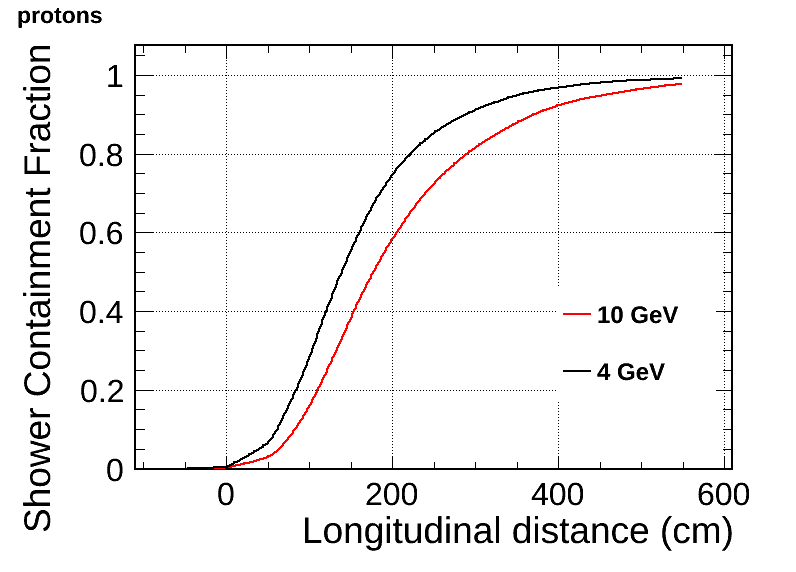
\includegraphics[width=0.49\textwidth,height=4.9cm]{figures/protons_lcont_overlay}&
   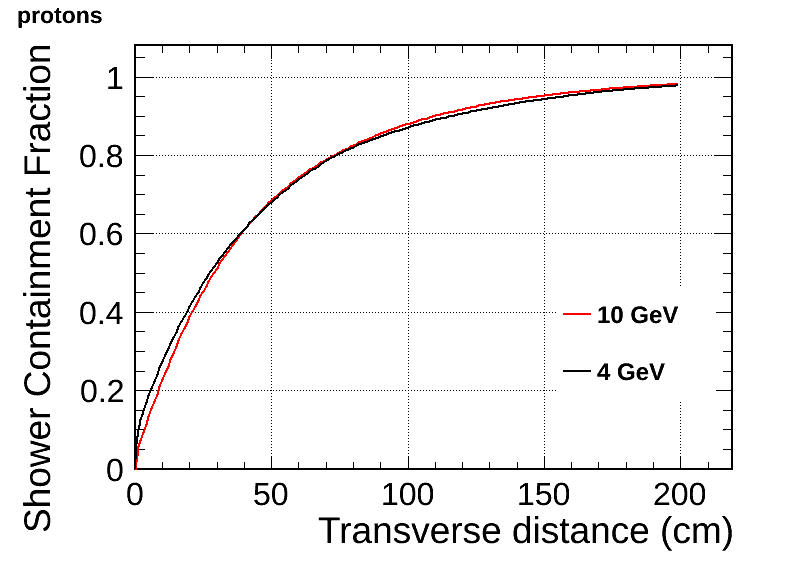
\includegraphics[width=0.49\textwidth,height=4.9cm]{figures/protons_wcont_overlay}\\
%    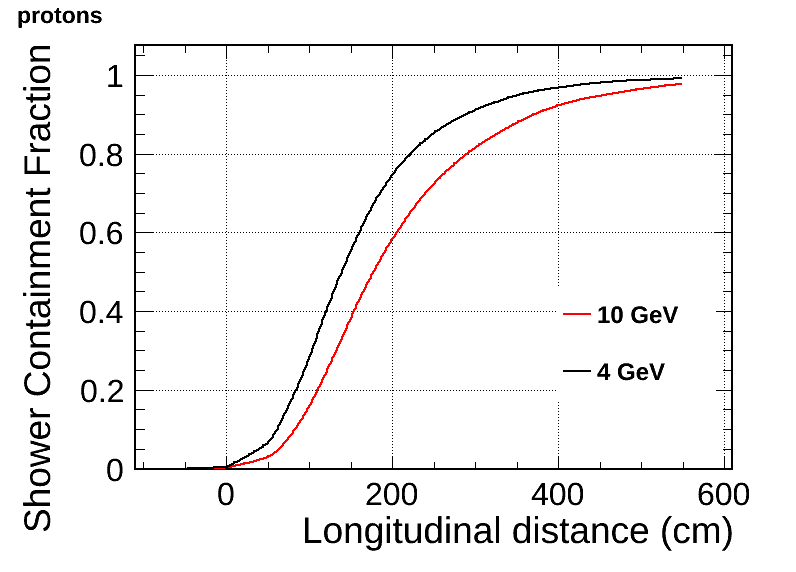
\includegraphics[scale=0.15]{figures/protons_lcont_overlay}&
%    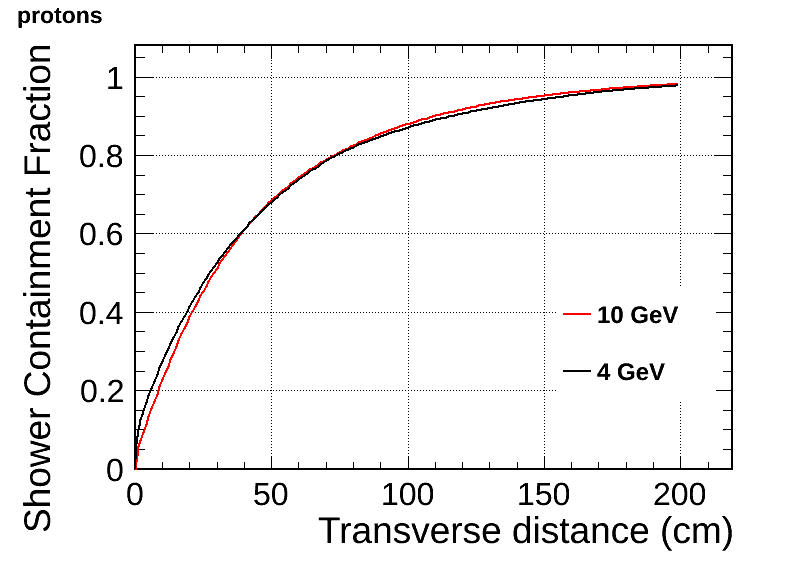
\includegraphics[scale=0.15]{figures/protons_wcont_overlay}\\
% 
%    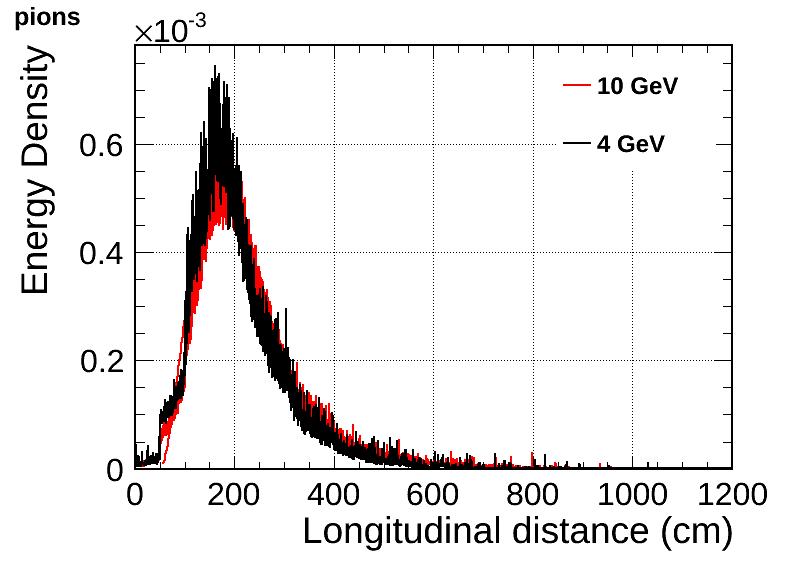
\includegraphics[scale=0.15]{figures/pions_density_overlay}&
%    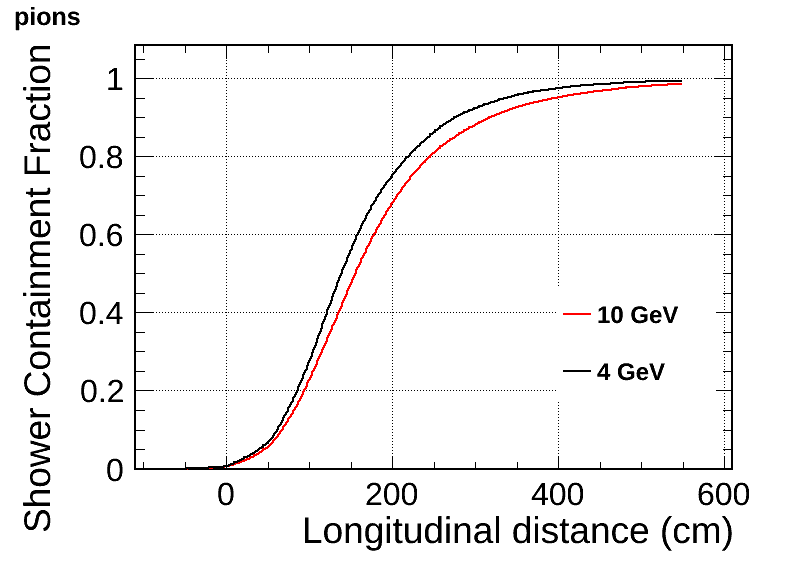
\includegraphics[scale=0.15]{figures/pions_lcont_overlay}&
%    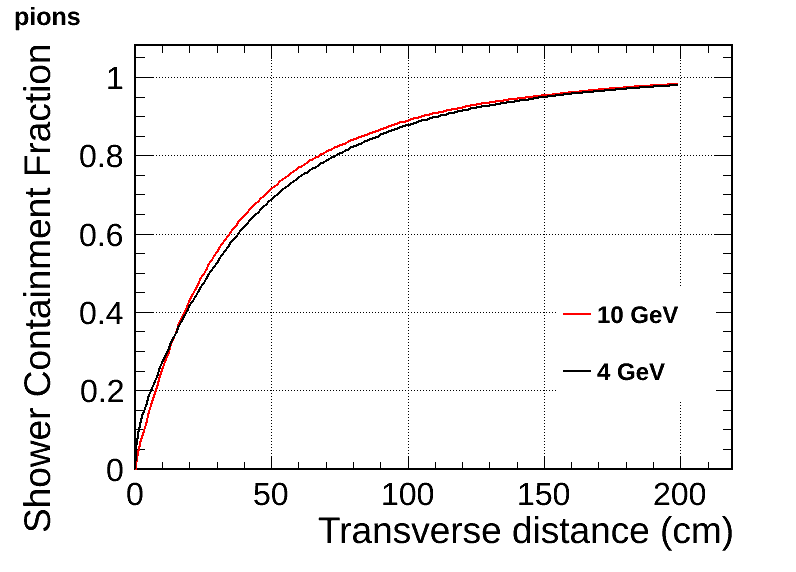
\includegraphics[scale=0.15]{figures/pions_wcont_overlay}\\
 
%   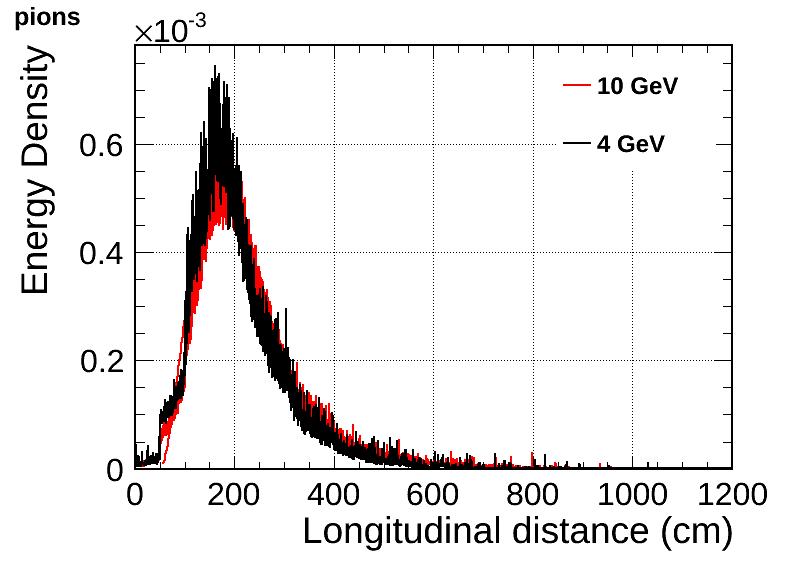
\includegraphics[width=0.31\textwidth,height=3.5cm]{figures/pions_density_overlay}&
%   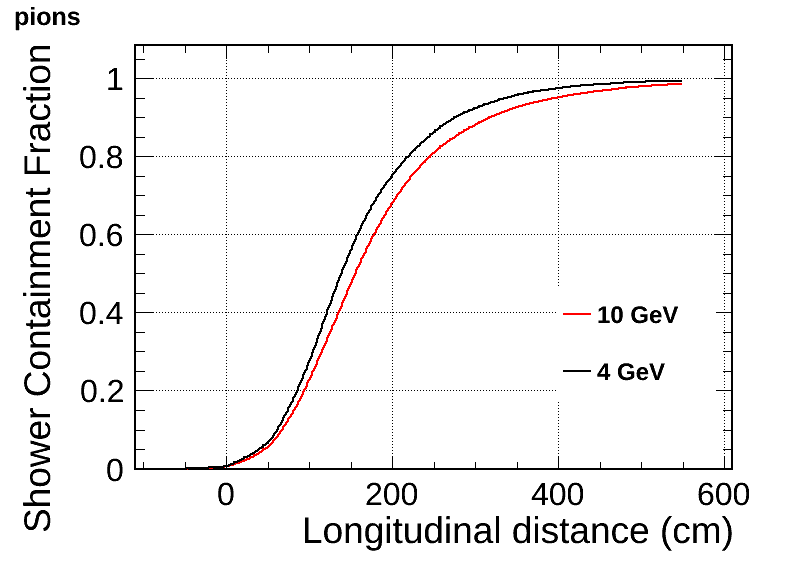
\includegraphics[width=0.31\textwidth,height=3.5cm]{figures/pions_lcont_overlay}&
%   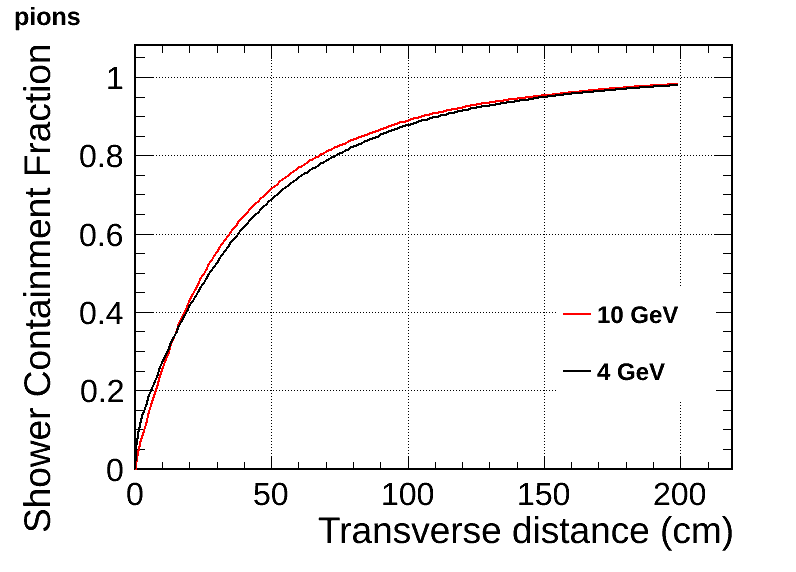
\includegraphics[width=0.31\textwidth,height=3.5cm]{figures/pions_wcont_overlay}\\
%    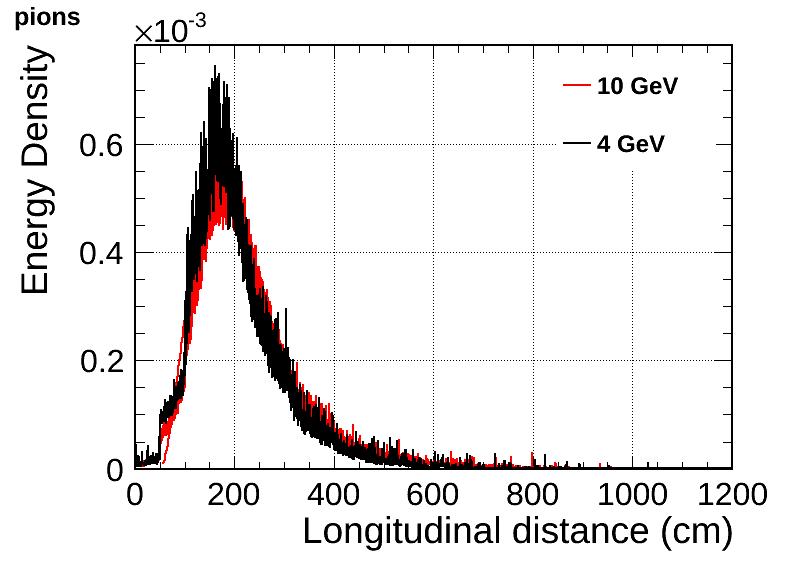
\includegraphics[scale=0.15]{figures/pions_density_overlay}&
%    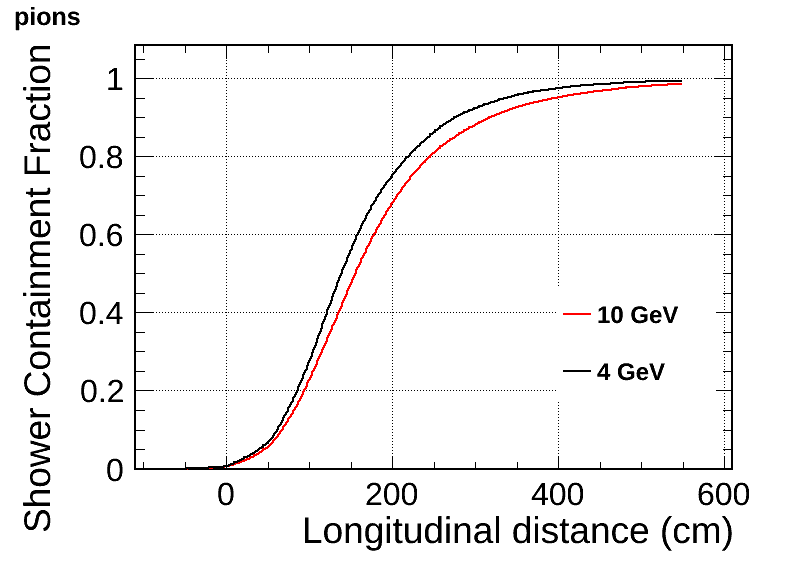
\includegraphics[scale=0.15]{figures/pions_lcont_overlay}&
%    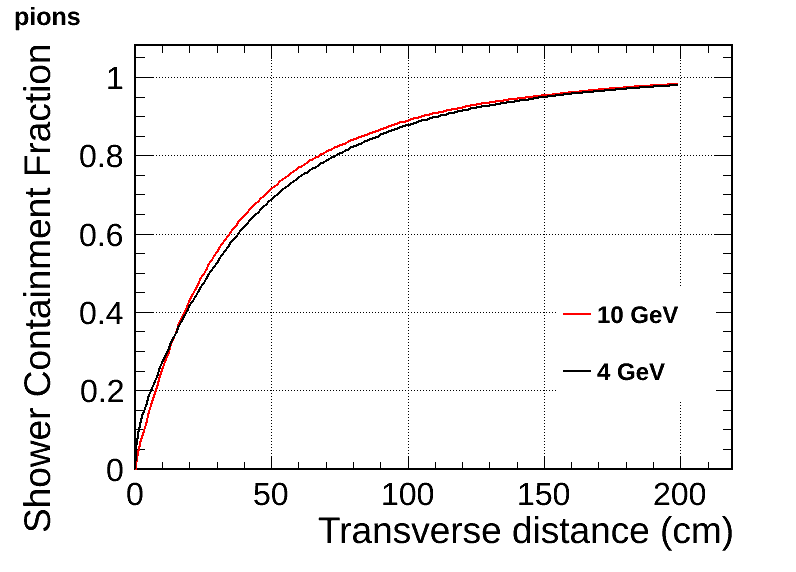
\includegraphics[scale=0.15]{figures/pions_wcont_overlay}\\
 
% 
%    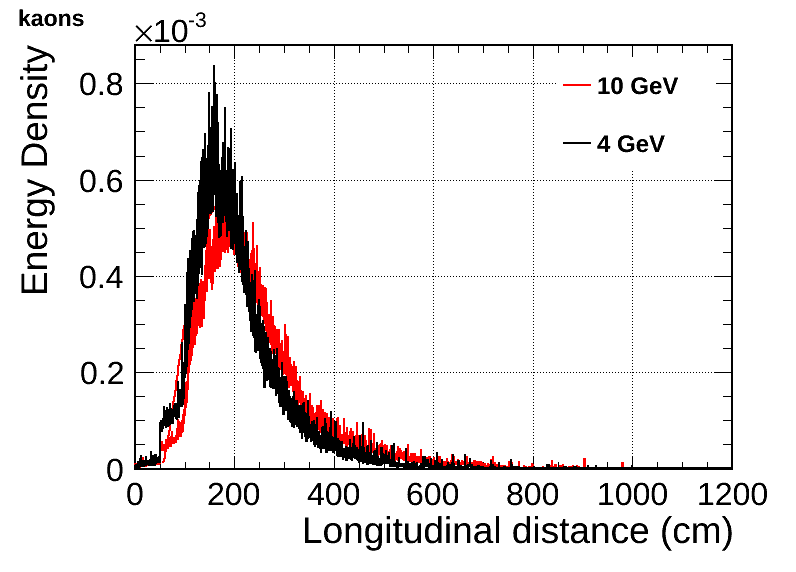
\includegraphics[scale=0.15]{figures/kaons_density_overlay}&
%    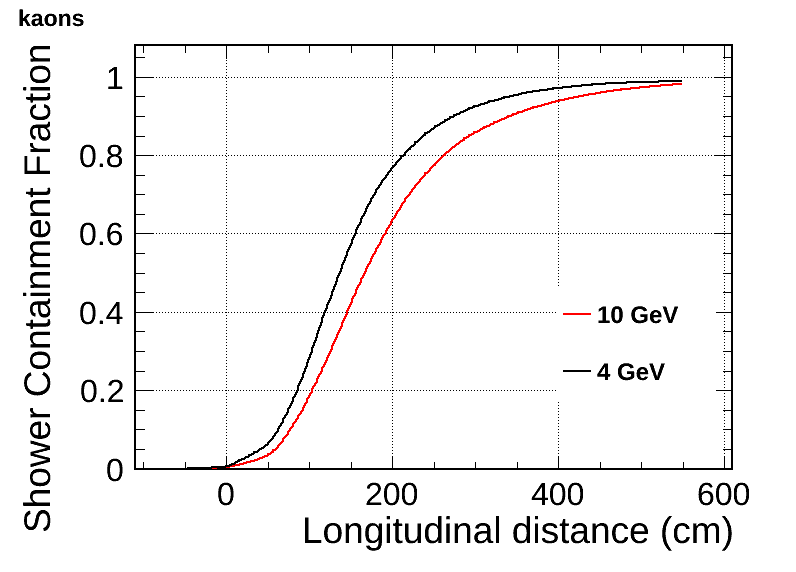
\includegraphics[scale=0.15]{figures/kaons_lcont_overlay}&
%    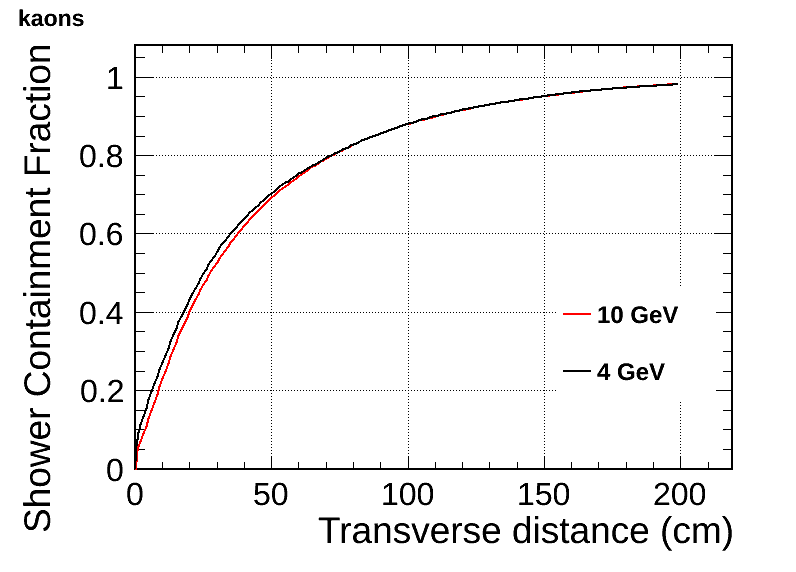
\includegraphics[scale=0.15]{figures/kaons_wcont_overlay}\\
 
  \end{tabular}
  \caption{Simulated longitudinal and transverse containment for proton showers of 4 and 10~GeV/c momenta.
%{\color{red}
%Improve or perhaps remove far left plot (binning too fine).
%Add info on simulation details and containment defn (T. Junk).
%}
}
%For 10 GeV showers, more than 95\% of the energy is contained in a detector of longitudinal size of 550~cm and 
%radius of 200~cm.}
\end{figure}

%\clearpage
%\subsubsection{Particle rates}
%\label{detbeam_rates}
%Estimation of  beam particles rates  necessary to collect high enough statistics in a reasonable time to obtain goals of of the measurements.
% THis should be discussed in the beam section
\subsubsection {Summary of Beam Particle Requirements}

Table~\ref{tab:runsum} summarizes the requested particle types and momenta along with 
required exposures for the test beam program.
\begin{table}[h]
\centering
\begin{tabular}{|c|c|c|l|}
\hline
Particle & Momenta (GeV/c) & Exposure & Purpose \\ \hline
$\pi^+$       & 0.2, 0.3, 0.4, 0.5, 0.7, 1, 2, 3, 5, 7     &  10K  & hadronic cal, $\pi^0$ content \\ \hline
$\pi^-$       &  0.2, 0.3, 0.4, 0.5, 0.7, 1     &  10K  & hadronic cal, $\pi^0$ content \\ \hline
$\pi^+$   &  2  &  600K & $\pi^o$/$\gamma$ sample \\ \hline
%$\pi^+$ &   1 \& 2  &  10K  & vary angle ($\times$5), reco \\ \hline
e$^+$ or e$^-$       &    0.2, 0.3, 0.4, 0.5, 1, 2, 3, 5, 7        &    10K   & e-$\gamma$ separation/EM shower     \\ \hline
% e$^+$ or e$^-$  &  1 \& 2  &  10K  & vary angle($\times$5), reco \\ \hline
%e$^+$ or e$^-$   (w/rad) &  3  &  20K  & tagged photons \\ \hline
$\mu^-$  &   (0.2), 0.5, 1, 2  &  10K & $E_\mu$, Michel el., charge sign \\ \hline
$\mu^+$ &   (0.2), 0.5, 1, 2   &  10K & $E_\mu$, Michel el.,charge sign  \\ \hline
$\mu^-$ or $\mu^+$ &   3, 5, 7  &  5K & $E_\mu$ MCS \\ \hline
%$\mu^-$ or $\mu^+$  &  1 \& 2  &  5K  & vary angle ($\times$5), reco \\ \hline
proton &  0.7, 1, 2, 3   &  10K & response, PID \\ \hline
proton &  1   &  1M & mis-ID pdk, recombination \\ \hline
%proton &  1 \& 2 &  10K & vary angle ($\times$5), reco \\ \hline
antiproton &  low-energy tune  &  (100) & antiproton stars \\ \hline
K$^+$  & 1 & (13K)   &   response, PID, PDK  \\ \hline
K$^+$  & 0.5, 0.7 & (5K)   &   response, PID, PDK  \\ \hline \hline
$\mu$, e, proton  & 1 (vary angle $\times$5 & 10K  & reconstruction  \\ \hline
\end{tabular}
\caption{Requirements summary for particle types and momenta. Items in parenthesis indicate lower priority (see text).
}
\label{tab:runsum}
\end{table}



%Charged pion samples will be used to characterize hadronic shower response and to measure
%absorption cross section parameters on argon.
%for all energies except 0.1 GeV point). 
%Muon samples will be used for calibration and 
%reconstruction tests. Electron samples will be used to measure EM shower response  
%and to tune PID algorithms (statistics shown will far exceed 1\% uncertainty on the mean for 
%EM showers with resolution on the order of 1\% as measured in DOCDB 9434 and 8835. 100k Electron event samples will allow
%high statistics studies of e-gamma separation).  
%Proton response will be studied for reconstruction and to tune PID 
%algorithms. Kaon data will be needed to tune proton decay backgrounds .
%Special runs at various angles with $\pi$, $\mu$, p and electrons will be performed to study reconstruction and tune PID algorithms. 

\subsection{Detector performance tests}

The prototype detector will allow to study the detector response to charge particles from the test beam. The measured energy deposition for various particles and its dependence on the direction of the particle will be used to tune
Monte Carlo simulations and allow more precise reconstruction of neutrino energy and interactions topologies with good particle identification.


\subsubsection{Shower calibration}

Accurate measurement of neutrino energy will require reconstruction of both electromagnetic and hadronic showers. Reconstruction of hadron energy 
in this energy range will require knowledge of the initiating hadron's 
($\pi^{+/-}$, $p$, or $K^{+/-}$)
fate (interact, decay, or stop). For the case of  interacting hadrons 
the composition of secondaries, which will include neutrals, particles which 
deposit energy electromagnetically ($\pi^o$, $\gamma$), as well as 
secondary hadrons,
%and their energy responses 
will need to be determined to characterize the response. 
The test beam with know incoming particle type and momentum will be used
to characterize interacting hadrons in this energy range.
%quantify responses to initiating hadrons
%($\pi^{+/-}$, $p$, or $K^{+/-}$)
%Hadronic showers initiated by protons in this energy range require

Fig.~\ref{fig:hadronshwr} shows the fraction of true energy deposited by interacting protons with 1~GeV/c (left) and
3~GeV/c (right) incident momenta simulated using FLUKA~\cite{fluka}. 65\% of protons with 1~GeV/c will interact while the remaining 
35\% will range out (see Sec.~\ref{dedx}). The resulting energy deposition in the two cases cannot be 
accurately characterize by an average shower calibration factor. Monte Carlo simulations of 
outgoing particles, especially at low energies) must be checked and bench marked against calibration data to avoid
large uncertainties from shower modeling. 
\begin{figure}[h!]
  \centering
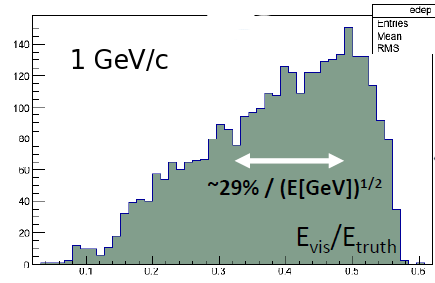
\includegraphics[width=0.49\textwidth,height=5.0cm]{figures/protons_1gev_v0}
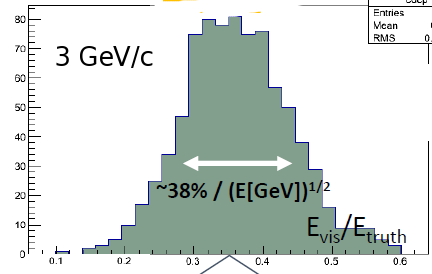
\includegraphics[width=0.49\textwidth,height=5.0cm]{figures/protons_3gev_v0}
\label{fig:hadronshwr}
  \caption{Fraction of true energy deposited by interacting protons of 1~GeV/c (left) and
3~GeV/c (right) momenta simulated using FLUKA~\cite{fluka}.
{\color{red}
Place holders cut from March workshop talk R\&D - Need better versions.
}
}
\end{figure}

Pion showers at low energies will also be important both for determining the interacted neutrino energy as well
as for modeling neutral current backgrounds resulting from $\pi^o$ content in showers. Differences in energy deposited
by $\pi^+$ versus $\pi^-$ initiated interactions are present up to momenta on the order of 1~GeV/c due to different
final state particles and interaction cross sections. This is illustrated in 
Fig.~\ref{fig:pionshwr} which shows the differences in mean energy deposited (left) and width (right) 
for interacting pions ranging from 0.2~GeV/c up to 7~GeV/c momenta simulated using FLUKA(?).
There is a strong case~\ref{lariat,T2K} for improving 
knowledge of exclusive final states and interaction cross section at low energies. Test beam samples
will be used both to study exclusive interaciton cross sections and to characterize energy deposition 
patterns for interacting  $\pi^+$ and $\pi^-$.
\begin{figure}[h!]
  \centering
%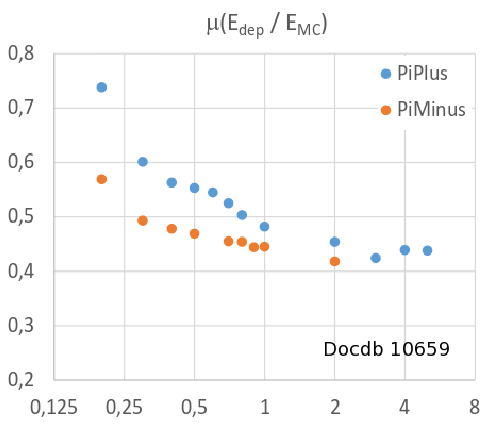
\includegraphics[width=0.49\textwidth,height=5.0cm]{figures/pi+pi-_means}
%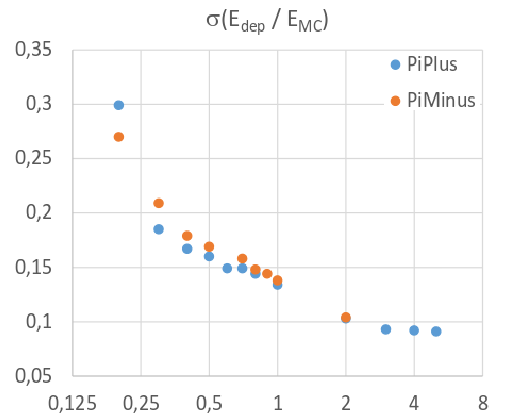
\includegraphics[width=0.49\textwidth,height=5.0cm]{figures/pi+pi-_sig}
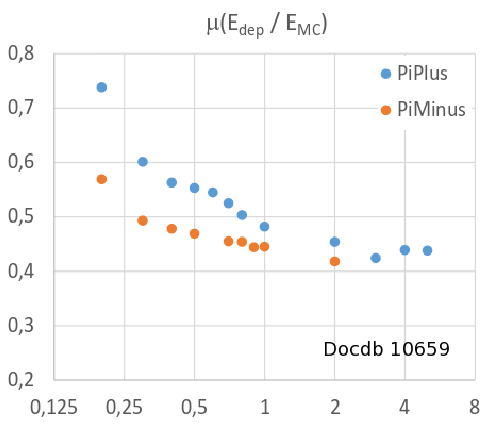
\includegraphics[width=0.49\textwidth,height=5.0cm]{figures/pi+pi-_means}
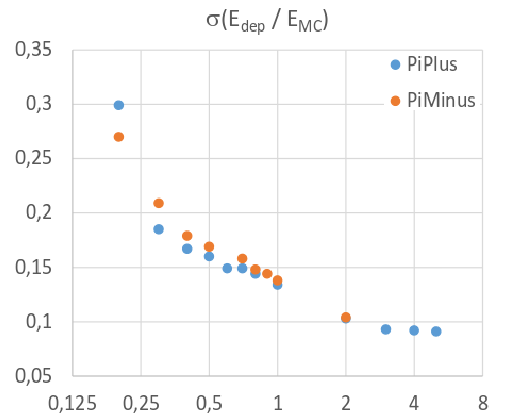
\includegraphics[width=0.49\textwidth,height=5.0cm]{figures/pi+pi-_sig}
\label{fig:pionshwr}
  \caption{Differences in mean energy deposited (left) and width (right) 
for interacting pions ranging from 0.2~GeV/c up to 7~GeV/c momenta simulated using FLUKA(?).
{\color{red}
Place holders cut from DOCDB 10659  - Need better versions.
}
}
\end{figure}


% 
%\begin{table}[h]
%\centering
%\begin{tabular}{|c|c|c|}
%\hline
%Particle     & Momenta (GeV)                                                                                       & Exposure/bin (total)  \\ \hline
%$\pi ^+ $   & 0.2-1.0 (100MeV bins), 1.0-10.0 ( 200MeV bins)    &  1000 (48k)     \\ \hline
%$\pi ^- $    & 0.2-1.0 (100MeV bins), 1.0-10.0 ( 200MeV bins)    &  1000 (48k)     \\ \hline
%$e^+$       & 0.2-10  (100MeV bins), 1.0-10.0 ( 200MeV bins)    &  1000 (48k)       \\ \hline
%$e^- $       & 0.2-10  (100MeV bins), 1.0-10.0 ( 200MeV bins)    &  1000 (48k)       \\ \hline
%$\mu^+$   & 0.2-1.0 (100MeV bins), 1.0-10.0 ( 200MeV bins)    &  1000 (48k)     \\ \hline
%$\mu^-$    & 0.2-1.0 (100MeV bins), 1.0-10.0 ( 200MeV bins)    &  1000 (48k)     \\ \hline
%$p$          &  0.2-1.5 (100MeV bins), 1.5-10.0 ( 200MeV bins)    &  1000 (56k)     \\ \hline
%$\bar p$   &  0.2-1.5 (100MeV bins), 1.5-10.0 ( 200MeV bins)    &  1000 (56k)     \\ \hline
%$K^+$      &  0.2-1.5 (100MeV bins), 1.5-10.0 ( 200MeV bins)    &  1000 (56k)     \\ \hline
%$K^- $      &  0.2-1.5 (100MeV bins), 1.5-10.0 ( 200MeV bins)    &  1000 (56k)     \\ \hline
%\end{tabular}\caption{Data sample requirements for shower calibrations.  Currently about 1k particles is assumed per bin to include variations in the shower topologies. Details MC analysis is necessary. }
%\end{table}
%


\subsubsection{Cross section measurements}
WIP from Jarek\\

Precise measurement of the  absorption and charge exchange of pions and kaons. Pion absorption is a large part of the pion nucleon cross section from 50 MeV to 500MeV with no data above about 1GeV pion kinetic energy. 
{\bf Add plots and values for known cross sections wit errors} 
\begin{itemize}
\item pion absorption on argon - Kotlinski, EPJ 9, 537 (2000)
\item pion cross section as a function of A - Gianelli PRC 61, 054615 (2000)
\end{itemize}
There is not currently a satisfactory theory describing absorption. The Valencia group (Vicente-Vacus NPA 568, 855 (1994)) developed model of    the pion-nucleus reaction with fairly good agreement, although not in detail. The actual  mechanism of multi-nucleon absorption
 is not well understood. 
 


\subsubsection{Bethe-Bloch parametrization of charged particles and PID}



%\begin{table}[h]
%\centering
%\begin{tabular}{|c|c|c|}
%\hline
%Particle     & Momenta (GeV)                                                                                       & Exposure/bin (total)  \\ \hline
%$\pi ^+ $   & 0.2-1.0 (50MeV bins), 1.0-3.0 ( 100MeV bins), 3.0-10 ( 200MeV bins)    &  200 (16.6k)     \\ \hline
%$\pi ^- $    & 0.2-1.0 (50MeV bins), 1.0-3.0 ( 100MeV bins), 3.0-10 ( 200MeV bins)    &  200 (16.6k)     \\ \hline
%$e^+$       & 0.2-10  (200MeV bins)                                                                              &  200 (9.8k)        \\ \hline
%$e^- $       & 0.2-10  (200MeV bins)                                                                              &  200 (9.8k)        \\ \hline
%$\mu^+$   & 0.2-1.0 (50MeV bins), 1.0-3.0 ( 100MeV bins), 3.0-10 ( 200MeV bins)    &  200 (16.6k)    \\ \hline
%$\mu^-$    & 0.2-1.0 (50MeV bins), 1.0-3.0 ( 100MeV bins), 3.0-10 ( 200MeV bins)    &  200 (16.6k)     \\ \hline
%$p$          &  0.2-1.5 (50MeV bins), 1.5-3.0 ( 100MeV bins), 3.0-10 ( 200MeV bins)    &  200 (17.2k)     \\ \hline
%$\bar p$   &  0.2-1.5 (50MeV bins), 1.5-3.0 ( 100MeV bins), 3.0-10 ( 200MeV bins)    &  200 (17.2k)    \\ \hline
%$K^+$      &  0.2-1.5 (50MeV bins), 1.5-3.0 ( 100MeV bins), 3.0-10 ( 200MeV bins)    &  200 (17.2k)      \\ \hline
%$K^- $      &  0.2-1.5 (50MeV bins), 1.5-3.0 ( 100MeV bins), 3.0-10 ( 200MeV bins)    &  200 (17.2k)    \\ \hline
%\end{tabular}\caption{Data sample requirements for the $dE/dx$ Bethe-Bloch parametrisation. The lower range starts with the nominal 200 MeV which is not achievable for p and difficult for K. The rough estimate is that we need about 200 particles per bin assuming that about half of them will be actually measured it gives  10\% statistical error for each bin but lower for the fit to the Bethe-Bloch formula. About half of the data sample is in the high momenta region, which can be reduce by decreasing number of particles per bin. }
%\end{table}
%


\label{detbeam_pid}

%The reconstruction of events in the LAr TPC is still a challenge but rapid progress has been achieved in recent years (cite pandora and other reconstruction algorithms). Despite the progress reconstruction algorithms have to rely Monte Carlo predictions which don't simulate liquid argon detectors responses correctly. Reconstruction algorithms will benefit greatly from test beam data particularly from the full scale prototype. The reconstruction algorithms will be trained to correctly reconstruct track, electromagnetic and hadronic showers.
%The data of tracks and showers can be used to create a library of reference events with which to tune algorithms.
%which can be used for matching with he neutrino data, similar to the  LEM (library event matching).

Information on range and charge deposition for stopping charged-particles can be used to 
accurately identify particle type as well as measure kinetic energy. 
Fig.~\ref{fig:resrange}  (left) shows track energy loss per unit length (dE/dx) as a function of residual 
track range for muons, pions, protons and kaons. 
%ALSO include the plot of probabilities from Robert here.
Probability functions for each particle hypothesis are also shown. 
%The tail is used to calibration the MIP response, the region near the end of the track is used
%to give PID information. (WIP)
Test beam measurements of stopping particles of each type will be used
to calibrate the energy deposition functions and to determine particle 
mis-ID probabilities. 
\begin{figure}[h!]
  \centering
%\includegraphics[width=0.49\textwidth,height=5.0cm]{figures/pid}
%\includegraphics[width=0.49\textwidth,height=5.0cm]{figures/pid_probabilities}
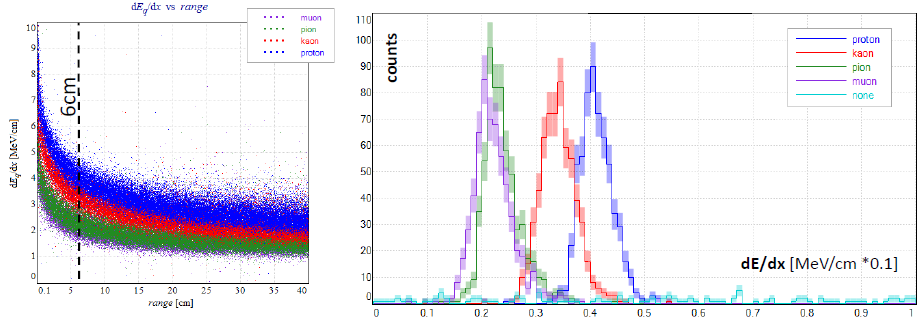
\includegraphics[width=\textwidth,height=5.0cm]{figures/pid_curves}
\label{fig:resrange}
  \caption{PID curves - residual range.
{\color{red}
Need better versions
}
}
\end{figure}


\subsubsection{Angular Dependence Effects}

Angular dependence of Recombination plots 


\subsubsection{Reconstruction Effects}



Main issues for the reconstruction algorithms:
\begin{itemize}
\item The reconstruction algorithms try to use all three planes on the signal readout. if the orientation of the track/shower is such that it is aligned with wires on one of the plans it significantly reduces quality of reconstructed objects. 
\item Calorimetry with collection and induction planes. In the ICARUS experiment the deposited energy was reconstructed from the signal on the collection plane. The induction planes bipolar signal wasn't "stable" enough to use it for calorimetric measurement. In the ELBNF design there is additional shielding  wire plane which will improve the quality of the bipolar signal and the  test beam experiment will help with its calibration.
\item   Vertexing.
\item Reconstruction efficiency for low energy particles. The reconstruction algorithm suffer from the lose of efficiency for low energy particle or particles which leave less than 200-300 hits. Training the algorithms on a low energy particles from the test beam will improve the quality and efficiency of the reconstructed objects.
\end{itemize}
%
%\begin{table}[h]
%\centering
%\begin{tabular}{|c|c|c|}
%\hline
%Particle     & Momenta (GeV)                                                                                       & Exposure/bin (total)  \\ \hline
%$\pi ^+ $   & 0.2-1.0 (100MeV bins), 1.0-10.0 ( 200MeV bins)    &  500 (26.5k)     \\ \hline
%$\pi ^- $    & 0.2-1.0 (100MeV bins), 1.0-10.0 ( 200MeV bins)    &  500 (26.5k)     \\ \hline
%$e^+$       & 0.2-10  (100MeV bins), 1.0-10.0 ( 200MeV bins)    &  500 (26.5k)       \\ \hline
%$e^- $       & 0.2-10  (100MeV bins), 1.0-10.0 ( 200MeV bins)    &  500 (26.5k)       \\ \hline
%$\mu^+$   & 0.2-1.0 (100MeV bins), 1.0-10.0 ( 200MeV bins)    &  500 (26.5k)     \\ \hline
%$\mu^-$    & 0.2-1.0 (100MeV bins), 1.0-10.0 ( 200MeV bins)    &  500 (26.5k)     \\ \hline
%$p$          &  0.2-1.5 (100MeV bins), 1.5-10.0 ( 200MeV bins)    &  500 (27.8k)     \\ \hline
%$\bar p$   &  0.2-1.5 (100MeV bins), 1.5-10.0 ( 200MeV bins)    &  500 (27.8k)     \\ \hline
%$K^+$      &  0.2-1.5 (100MeV bins), 1.5-10.0 ( 200MeV bins)    &  500 (27.8k)     \\ \hline
%$K^- $      &  0.2-1.5 (100MeV bins), 1.5-10.0 ( 200MeV bins)    &  500 (27.8k)     \\ \hline
%\end{tabular}\caption{Data sample requirements for the development of the reconstruction algorithms. The most important are  the low momenta particles where the showers are more likely to have different topologies. }
%\end{table}


\subsubsection{e/$\gamma$ separation}

The search for a CP violation phase using $\nu_e$ appearance 
in a $\nu_\mu$ beam requires good electron/photon separation.
Backgrounds originating from photons produced primarily from 
final state $\pi^0$'s must be identified and removed from the signal
electron sample. 


The photons can undergo two process: pair production and Compton scattering. 
The dominant process for photons with energies of several hundreds MeV  is 
the e$^+$ e$^-$ pair production, but Compton scattering also occur at this 
energies. For pair production the e/$\gamma$ separation is achieved by looking 
at the beginning of the electromagnetic shower, where for election we see energy 
deposition typical for single MIP and for photon we see energy deposition consisted 
with two MIPs. In case of Compton scattering off of atomic electrons the 
signal is much more difficult to distinguish from the CC $\nu_e$ scattering signal.

Electron-photon separation has been studied in LAr TPCs
(Icarus and Argoneut) as shown in Fig.~\ref{fig:egam1}.
Currently the 
separation efficiency is estimated to be at the level of of 94 \% (? cite and 
check the number). 
This may depend on particular features of the geometry including wire pitch, etc.
Therefore, it is critically important 
to study e/$\gamma$ separation in a prototype LAr TPC detector.
{\bf we need someone to look into this}



\subsection{Other measurements} 


\subsubsection{Supernova and Michel electrons}
The energies of the electrons coming from CC $\nu_e$ interactions from Supernova will be in the order of 10s of MeV. 
The beam test cannot offer such low energy electron, but one can use the Michel electrons form $'mu$ decay to cover these energies. The SK used the Michel spectrum to calibrate the absolute energy scale. 


%\begin{table}[h]
%\centering
%\begin{tabular}{|c|c|c|}
%\hline
%Particle     & Momenta (GeV/c)    & Exposure/bin  \\ \hline
%$\mu^+$   & (0.2), 0.5, 1      &  10K    \\ \hline
%\end{tabular}\caption{Stopping . }
%\end{table}


\subsubsection{Charge sign determination}
It is not possible to determine charge of the particle on the event by event basis with non-magnetized LAr TPC detectors. A statistical separation will be studied which will make use of differences in muon versus antimuon capture cross sections and lifetime.
%However, the statistical analyst will be possible. We will fit the muon's half time which is different for muons and antimony due to different muon capture cross sections. 
For the $\mu^+$ for argon we expect about xx\% to be captured and for $\mu^-$ about yy\%. 




\subsubsection{Proton decay sensitivity and background samples}


The DUNE experiment in the deep underground location will improve sensitivity to detection of several modes of proton decay.
In particular, a first ever LAr detector of this scale underground will primarily improve sensitivity to 
proton decays with final state kaons such as  $p \rightarrow K^+ \overline{\nu}$. 
Sensitivity to this process is studied in \cite{bueno}. $K^+$ detector efficiencies are estimated to be $>$97\% in the
appropriate momentum range (500-800 MeV/c). The kaon samples requested in Table~\ref{pdktable} are needed to directly measure 
$K^+$ PID and detection efficiencies. Obtaining low energy kaons will likely be difficult in this beamline.
A sample of 13K beam kaons with 1~GeV/c momentum are requested to provide 2K stopping $K^+$ track samples for PID studies.
(only 15\% of $K^+$ at 1 GeV stop at 1~GeV/c).


\begin{table}[h]
\centering
\begin{tabular}{|c|c|c|}
\hline
Particle     & Momenta (GeV/c) & Exposure/bin  \\ \hline
\hline
K$^+$  &  1 & (13k)    \\ \hline
K$^+$  & 0.5, 0.7 & (5k)   \\ \hline
proton &  1  &  (1M)  \\ \hline
\end{tabular}\caption{Samples related to proton decay physics requirements.}
\label{pdktable}
\end{table}

A sizable sample of protons ($\sim 10^6$)
are requested to study the possible background contributions to  $p \rightarrow K^+ \overline{\nu}$.
This sample of  protons are needed to quantify the possibility that an interacting {\bf p} 
is  {\em mis-IDed as stopping K}. A proton interaction which produces neutrals and one charged pion 
(which is mis-IDed or subsequently decays to $\mu$) can fake the final state kaon signal.


\subsubsection{Anti-proton annihilation }

A sample of antiproton would be useful to calibrate the $p$-$\overline{p}$ annihilation process. 
This would provide input to exotic B-violating process neutron oscillation (reference) modeling of 
subsequent  $n$-$\overline{n}$ annihilation. These events would be tagged in the mixed-mode beam.
Events should be at the lowest energies achievable in this beamline.



